\documentclass{beamer}
\hypersetup{pdfpagemode=FullScreen}
\usepackage{fontspec}
\usepackage{tcolorbox}
\tcbuselibrary{minted,skins}
\usepackage{graphicx}
\graphicspath{ {./images/} }

\newtcblisting{jscode}{
  listing engine=minted,
  colback=codebg,
  colframe=codebg,
  listing only,
  minted style=monokai,
  minted language=jsx,
  left=1mm,
}
\newtcblisting{jscodesmall}{
  listing engine=minted,
  colback=codebg,
  colframe=codebg,
  listing only,
  minted style=monokai,
  minted language=jsx,
  minted options={fontsize=\tiny},
  left=1mm,
}
\newtcblisting{bashcode}{
  listing engine=minted,
  colback=bashbg,
  colframe=bashbg,
  listing only,
  minted style=native,
  minted language=bash,
  minted options={linenos=true,texcl=true},
  left=1mm,
}
\definecolor{codebg}{rgb}{0.2,0.2,0.2}
\definecolor{bashbg}{rgb}{0.85,0.85,0.85}

\setsansfont{Open Sans}

\usetheme{metropolis}           % Use metropolis theme
\title{Lesson 2: Exploring React Native}
\subtitle{File Hierarchy, Flow and more}
\date{\today}
\author{Karl Steven Velasco Orjalo}
\institute{React Native Quickstart}

\begin{document}
\metroset{block=fill}
  \maketitle

  \begin{frame}{Lesson Outline}
    \setbeamertemplate{section in toc}[sections numbered]
    \tableofcontents
  \end{frame}

  \section{React Native's Structure}
  \begin{frame}[fragile]
    \frametitle{Taking a look at myNewProject}
    Open up myNewProject with VSCode from Open Folder. 
    We now see the standard structure of React Native.

    Over the course of a project, we will mostly only be working with the following:
    \begin{itemize}
      \item ./App.js
    \end{itemize}

    and additionally, create the following folders:
    \begin{itemize}
      \item ./src/pages/
      \item ./src/components/
      \item ./src/styles/
    \end{itemize}

    That's it! (again, mostly.)
  \end{frame}
  \begin{frame}
    \frametitle{Taking a look at myNewProject (cont.)}
    \begin{columns}[onlytextwidth]
      \begin{column}{0.4\textwidth}
        Your project structure should now look like this:
      \end{column}
      \begin{column}{0.6\textwidth}
        \centering
        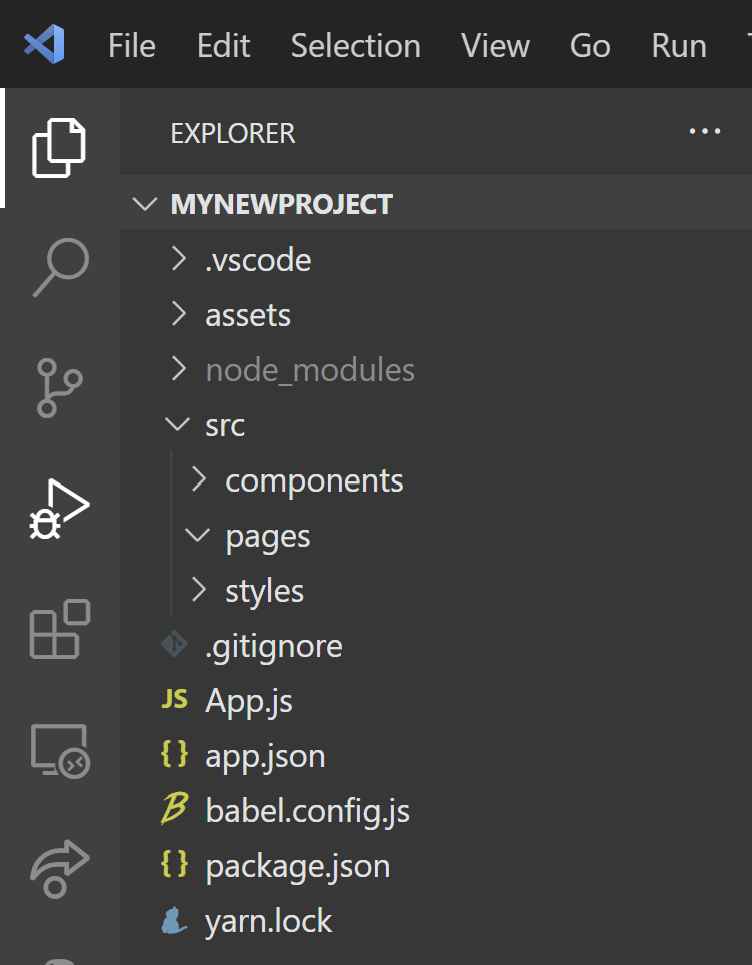
\includegraphics[scale=0.4]{structure}
      \end{column}
    \end{columns}
  \end{frame}

  \section{Creating blank pages with Bottom Bar Navigation}
  \begin{frame}[fragile]
    \frametitle{Making two blank pages}
    First, under \verb|./src/pages/|, create a file called \verb|home.jsx|.
    \begin{jscode}
import React from 'react'
import {View, Text} from 'react-native'

const Home = () => {
  return (
    <View>
      <Text>This is the Home page.</Text>
    </View>
  )
}

export default Home
    \end{jscode}

  \end{frame}
  \begin{frame}[fragile]
    \frametitle{Making two blank pages (cont.)}
    Next, under \verb|./src/pages/|, create a second file called \verb|Account.jsx|.
    \begin{jscode}
import React from 'react'
import {View, Text} from 'react-native'

const Account = () => {
  return (
    <View>
      <Text>This is the Account page.</Text>
    </View>
  )
}

export default Account
    \end{jscode}

  \end{frame}

  \begin{frame}[fragile]
    \frametitle{Making a Bottom Bar Navigator}
    We will now make these two pages accessible to the user through a Bottom Bar. 
    In \verb|./App.js| enter the code shown in the next two slides.
    \begin{jscodesmall}
import { createBottomTabNavigator } from "@react-navigation/bottom-tabs";
import { NavigationContainer, StackActions } from "@react-navigation/native";
import { SafeAreaProvider } from "react-native-safe-area-context";

// Import pages
import Home from './src/pages/home';
import Account from './src/pages/account';

// Create the Bottom Tab
const Tab = createBottomTabNavigator();
    \end{jscodesmall}

  \end{frame}

  \begin{frame}[fragile]
    \frametitle{Making a Bottom Bar Navigator (cont.)}
    \begin{jscodesmall}
const App = () => {
  return (
    // Avoid things like notches with SafeAreaProvider
    <SafeAreaProvider>
      <NavigationContainer>
        <Tab.Navigator>
          <Tab.Screen name = "Home" component={Home}></Tab.Screen>
          <Tab.Screen name = "Account" component={Account}></Tab.Screen>
        </Tab.Navigator>
      </NavigationContainer>
    </SafeAreaProvider>
  );
}

export default App
    \end{jscodesmall}
  \end{frame}
  
  \section{Running React Native}
  \begin{frame}[fragile]
    \frametitle{Installing Dependencies/Libraries}

    Before we run our app, we have used external Dependencies in \verb|./App.js|. 
    We will now install them with Yarn in our Terminal. 

    \begin{bashcode}
$ yarn add @react-navigation/bottom-tabs
$ yarn add @react-navigation/native
$ yarn add react-native-safe-area-context
    \end{bashcode}
  \end{frame}

  \begin{frame}[fragile]
    \frametitle{Running our app with Expo Go}

    With Expo Go installed on our phone through the App Store or Play Store, we are now ready to run our app.
    Enter the following command into your Terminal.

    \begin{bashcode}
$ yarn expo start
    \end{bashcode}
  \end{frame}
  \begin{frame}[fragile]
    \frametitle{Running our app with Expo Go (cont.)}

    You should now see a QR code printed into your Terminal. 
    Scan it with Expo Go directly if you're on Android, else if you're on iOS use the Camera App.
  \end{frame}
  \appendix

  \begin{frame}[standout]
    End of Lesson

    {\small Questions? Reach out at:}
    {\footnotesize karlorjalo@gmail.com}
  \end{frame}

\end{document}